%! Author = Philipp Emmenegger
%! Date = 08/06/2021

\section{Clean Code}
\subsection{Fundamentals}
\subsubsection{YAGNI}
\textbf{YAGNI - You Aren't Gonna Need It}
\begin{itemize}
    \item Code, that has never been written, can not rot
    \item Less code means less complexity
    \item Agile Mindset
\end{itemize}

\subsubsection{KISS}
\textbf{KISS - Keep it simple, stupid!}
\begin{itemize}
    \item Simple code tends to be more readable
    \item If there are options - choose the simple one
    \item Beware of premature optimizations
\end{itemize}

\subsubsection{Names}
\textbf{Positive Characteristics}
\begin{itemize}
    \item Intention-revealing
    \item Pronounceable
    \item Searchable
    \item Length matches scope
    \item Classes named with nouns
    \item Methods start with verb
    \item Consistent
    \item Domain-terminology
\end{itemize}
\textbf{Things to avoid}
\begin{itemize}
    \item Disinformation
    \item Similarity
    \item Encoding
    \item Magic numbers
\end{itemize}

\subsubsection{Functions}
\textbf{Positive Characteristics}
\begin{itemize}
    \item Short
    \item Ascertainable (line length < screen width)
    \item Short parameter lists
    \item Name starts with verb
    \item Name reflects responsibility
    \item Single responsibility
    \item One level of abstraction
    \item Command or query
\end{itemize}
\textbf{Things to avoid}
\begin{itemize}
    \item Duplication (DRY)
    \item Indent level > 2
    \item Side effects
    \item Output arguments
    \item Return codes
    \item Inappropriate use of switch
    \item Inappropriate use of try .. catch
\end{itemize}

\subsubsection{Classes}
\textbf{Positive Characteristics}
\begin{itemize}
    \item Short > 200 lines
    \item Straightforward signature
    \item Named with a noun
    \item Name reflects responsibility
    \item Hiding information
    \item High cohesion
    \item Single responsibility (SRP, ISP)
    \item Open for extension
    \item Isolated from change (DIP)
\end{itemize}
\textbf{Things to avoid}
\begin{itemize}
    \item Tight coupling
    \item Talking to strangers
    \item God classes
    \item Manager classes
\end{itemize}

\textbf{Cohesion} is the degree to which the elements inside a class belong together.\\
High cohesion often correlates with loose coupling and vice verca:
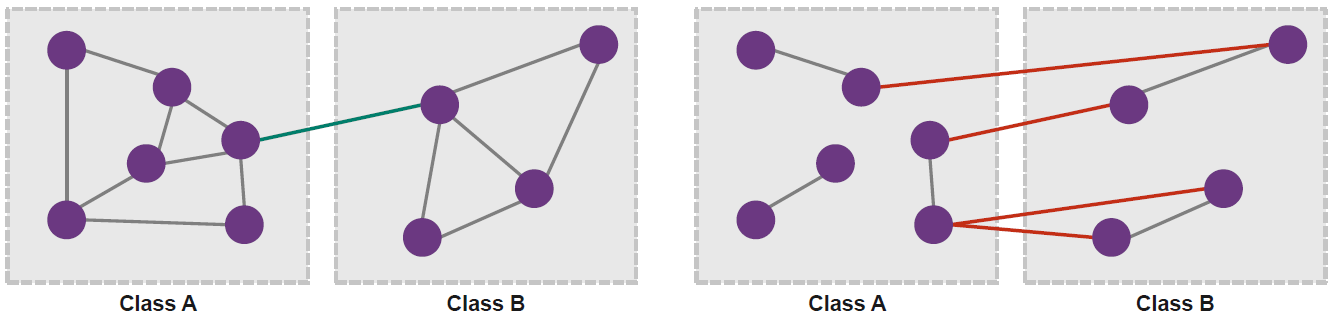
\includegraphics[width=\linewidth]{../img/cohesion.png}

\subsubsection{Classes - Law of Demeter}
\begin{itemize}
    \item Classes should not know the details of the objects it manipulates
    \item Don't talk to strangers!
    \item Tell, don't lie!
\end{itemize}
\begin{lstlisting}
car.getEngine().start();    // bad
car.prepareForRide();       // good
\end{lstlisting}

\subsubsection{Error Handling}
\begin{itemize}
    \item Use exceptions instead of error codes
    \item Add a precise description of the error
    \item Avoid returning null
\end{itemize}

\subsubsection{Comments}
\begin{itemize}
    \item Indicates bad code
    \item Instead of a comment, improve your code
    \item Very hard to maintain
    \item Can be misleading when outdated
    \item Add noise to the code
\end{itemize}
\textbf{Appropriate uses of comments:}
\begin{itemize}
    \item Explanation or information
    \item Warning of consequences
    \item Legal comments
    \item Highlight work in progress
\end{itemize}
\textbf{Things to avoid}
\begin{itemize}
    \item Redundant comments
    \item Extensive comments
    \item Misleading comments
    \item Mandated comments
    \item Jounal comments
    \item Position markers / seperators
    \item commented-out code
\end{itemize}

\subsection{Design Principles}
\subsubsection{DRY - Don't Repeat Yourself}
\begin{itemize}
    \item Duplication: primary enemy of maintainability
    \item Bugs must be fixed multiple times
    \item Features must be added multiple times
    \item Forget any copy and the nightmare begins
\end{itemize}

\subsubsection{OLA - One Level of Abstraction}
\begin{itemize}
    \item Keeping one level of abstraction fosters readability
    \item aka. Single Level of Abstraction
\end{itemize}
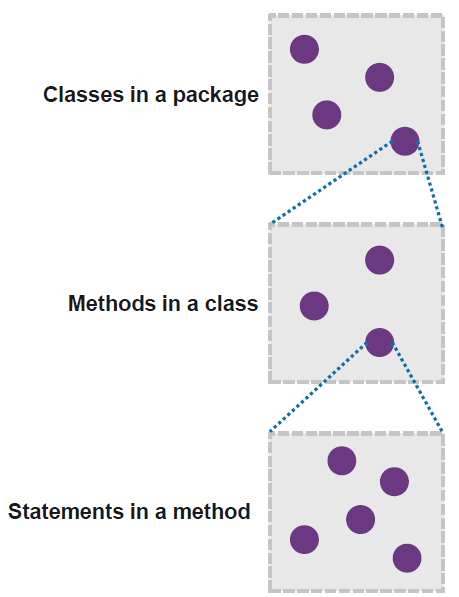
\includegraphics[width=0.5\linewidth]{../img/OLA.png}

\subsubsection{SRP - Single-Responsibility Principle}
\begin{itemize}
    \item A class, module or functio should have only one single reason to change
    \item Compose software of many small classes
\end{itemize}

\subsubsection{OCP - Open-Closed Principle}
\begin{itemize}
    \item Software entities should be open for extension but closed for modification
    \item Possible to add functionality without changing existing code
    \item Inheritance / Composition
\end{itemize}

\subsubsection{LSP - Liskov Substitution Principle}
\begin{itemize}
    \item Subtypes must behave like their base type
    \item A subtype may extend base type functionality but must not reduce it
\end{itemize}

\subsubsection{ISP - Interface Segregation Principle}
\begin{itemize}
    \item A client shall only depend on the details which it does use
    \item Extracting interfaces / super classes
    \item The leaner the service interface is, the smaller the coupling of both components
    \item Increased readability
\end{itemize}

\subsubsection{DIP - Dependency Inversion Principle}
\begin{itemize}
    \item High-level classes must not depend on low-level classes
    \item Low-level classes can be replaced
    \item Dependency Injection
\end{itemize}

\subsubsection{CQS - Command Query Separation}
\begin{itemize}
    \item Every method should either perform an action or a query that returns data
    \item Querying methods are side-effect free
\end{itemize}











